\documentclass[a4paper, 11pt]{article}
\usepackage[top=2cm, bottom=2cm, left=1.5cm, right=1.5cm]{geometry}
\usepackage[utf8]{inputenc}
\usepackage{amsmath, amsfonts, amssymb}
\usepackage{graphicx}
\usepackage[brazil]{babel}
\usepackage{indentfirst}
\usepackage[small,bf]{caption}



\begin{document}
%%%%%%%%%%%%%%%%%%%%%%%%%%%%%%%%Começo do documento%%%%%%%%%%%%%%%%%%%%%%%%

	\begin{enumerate}
	\item \textbf{Resumo}
\paragraph{}

	O movimento de um corpo em um meio viscoso é influenciado pela ação de uma força viscosa, $F_V$, proporcional à velocidade, $v$. No caso de esferas, assumindo velocidades baixas e um fluido homogêneo e infinito em todas as direções, chega-se a uma força de atrito dada pela lei de Stokes: $F_V = 6 \pi \eta rv$, onde $r$ é o raio da esfera e $\eta$ o coeficiente de viscosidade do meio. Se uma esfera de densidade maior que a de um líquido for solta na superfície do mesmo, no instante inicial a velocidade é zero, mas a força resultante acelera a esfera de forma que sua velocidade vai aumentando. Pode-se verificar que a velocidade aumenta não-uniformemente com o tempo e atinge um valor limite, que ocorre quando a força resultante for nula. As três forças que atuam sobre a esfera estão representadas na Fig. 1 e são, além da força viscosa, o peso da esfera, $P$, e o empuxo, $E$. Igualando a resultante dessas três forças a zero, obtém-se a velocidade limite, $v_L$:

$$ v_L = \dfrac{2}{9} \dfrac{\rho - \rho'}{\eta} g r^2 , $$

onde $\rho$ e $\rho’$ são as densidades da esfera e a densidade do meio, respectivamente, e $g$ é a aceleração da gravidade. A figura abaixo mostra esquematizado as forças que atuam na esfera de aço durante um dado momento de sua trajetória ao longo do tubo de vidro contendo mistura de glicerina e água:

		\begin{figure}[h]
		\centering
		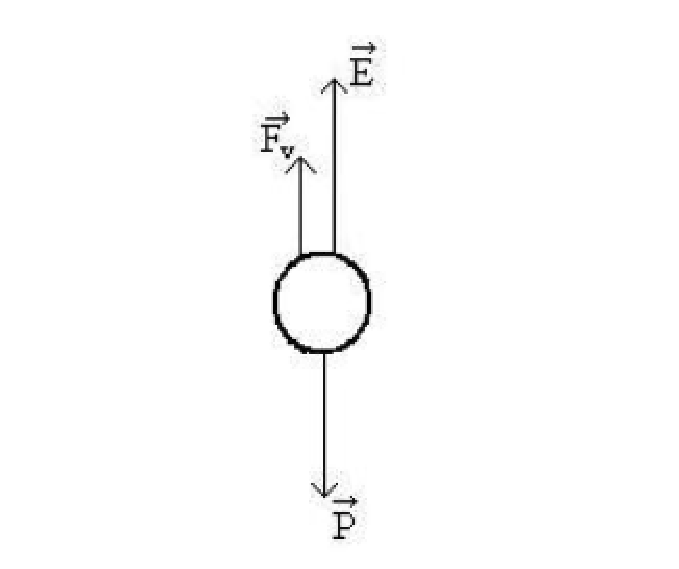
\includegraphics[scale = 0.5]{fig1.eps}
		\caption{Forças que atuam numa esfera num meio viscoso.}
		\end{figure}

\paragraph{}
No experimento dado, como as paredes do tubo de vidro são finitas, logo elas exerceram algum efeito sobre a esfera de aço, alterando a sua velocidade limite, fazendo com que ela não seja exatamente a velocidade da equação $v_L$ dada, então a equação com a correção dessa nova situação é dada da seguinte forma:
$$k \cdot v'_L = \dfrac{2}{9} \dfrac{\rho - \rho'}{\eta} g r^2 ,$$

onde 
$$k = (1 + 2,4 \cdot \dfrac{r}{R})(1 + 3,3 \cdot \dfrac{r}{H})$$
é decorrente do efeito de Ladenburgh, sendo $R$ e $H$, respectivamente, o raio do tubo e a altura total do fluído no tubo. Portanto, temos que multiplicar a velocidade limite da esfera no tubo, $v’_L$, por $k$, para se obter a velocidade limite prevista pela equação de $v_L$.
\pagebreak
	
	\item \textbf{Procedimentos e incertezas}
\paragraph{}
Para esse experimento utilizamos os seguintes aparatos: tubo de vidro com mistura de glicerina e água, suporte com marcas graduadas, conjunto de esferas, trena, paquímetro, micrômetro, cronômetro e termômetro de aço.

\begin{figure}[!h]
		\centering
		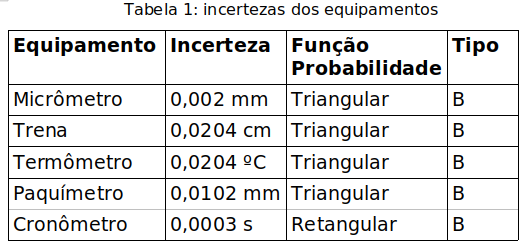
\includegraphics[scale = 0.45]{tabela1.png}
		%\caption{}
		\end{figure}

Nesse experimento fizemos uma atribuição de números as esferas com o intuito de identificação das mesmas ficando da seguinte forma: a esfera com diâmetro de 2,49 mm é (1), a esfera com diâmetro de 2,99 mm é (2), a esfera com diâmetro de 3,49 mm é (3) e a esfera com diâmetro de 3,95 mm é (4) - todos estes com o micrômetro. Medimos também, com uma trena, a altura da coluna da mistura de glicerina e água, obtendo a medida de 38 cm. Concomitante a isso, foi realizada a medição da temperatura, com um termômetro analógico, dessa mistura, obtendo-se 27ºC - medida feita no início e ao longo de intervalos de tempo espaçados. O procedimento experimental ficou definido pelo nosso grupo da seguinte maneira: dividimos as medições realizadas com as esferas em 4 grupos e para cada grupo foram realizadas 6 medidas do cronômetro (duas para cada membro do grupo, evitando a intensificação de erros considerados sistemáticos).
\\

\begin{figure}[!h]
		\centering
		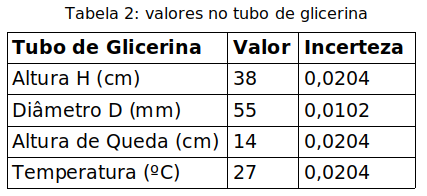
\includegraphics[scale = 0.45]{tabela2.png}
		%\caption{}
		\end{figure}

\textbf{OBS}: Durante a realização do experimento notamos a presença de uma película de água na superfície do líquido contendo a mistura de glicerina e água e isso foi devido a dissociação da água com a glicerina com o decorrer do tempo, logo as esferas foram soltas logo embaixo dessa película de água (recomendação do roteiro caso ocorresse esse fato).
\\

\textbf{Nota}: Em conjunto com a realização desse experimento, fizemos gravações através de um smartphone na resolução de 1920x1080p 60fps com o objetivo de analisar no \textit{Tracker} os dados coletados pelo nosso grupo para que possamos embasar nossas conclusões. Foram ao todo 24 vídeos gravados.
\\


	\item \textbf{Resultados}
\paragraph{}
Durante o experimento, foram feitas seis medidas de tempo de queda para cada esfera (duas por integrante), com o tamanho do percurso mantido constante ao longo de todo o experimento ($h = 140 +/- 0,2$ mm). Com isso, calculou-se a média dos tempos e suas respectivas incertezas combinadas, a fim de obter a velocidade-terminal média de cada lançamento. 
\pagebreak

\begin{figure}[!h]
		\centering
		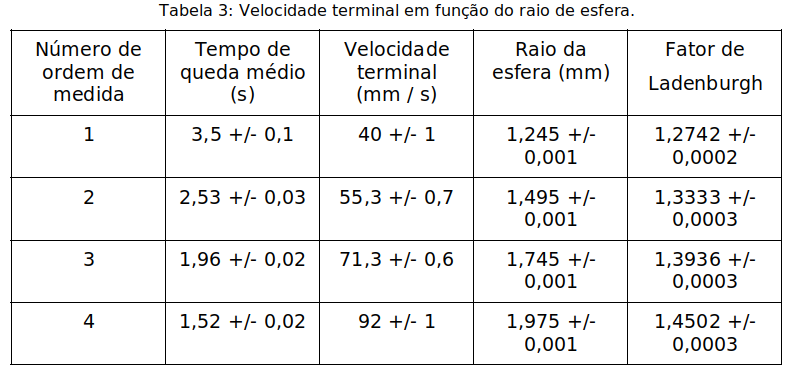
\includegraphics[scale = 0.35]{tabela3.png}
		%\caption{}
		\end{figure}

Com os raios das esferas, as velocidades-terminal e o fatores de Ladenburgh, podemos fazer a regressão linear e montar o gráfico linearizado com o \textit{software SciDAVis}. A equação $v'_L = \dfrac{2}{9} \dfrac{\rho - \rho'}{\eta} g \cdot \dfrac{r^2}{k}$ pode ser linearizada tomando a seguinte relação:
$ v'_L \longrightarrow y; $
$ \dfrac{2}{9} \dfrac{\rho - \rho'}{\eta} g \longrightarrow a $ e;
$ \dfrac{r^2}{k} \longrightarrow x $
que representa uma equação de uma reta do tipo $y = a \cdot x$, teoricamente centrada na origem.
\\

\begin{figure}[htb]
		\centering
		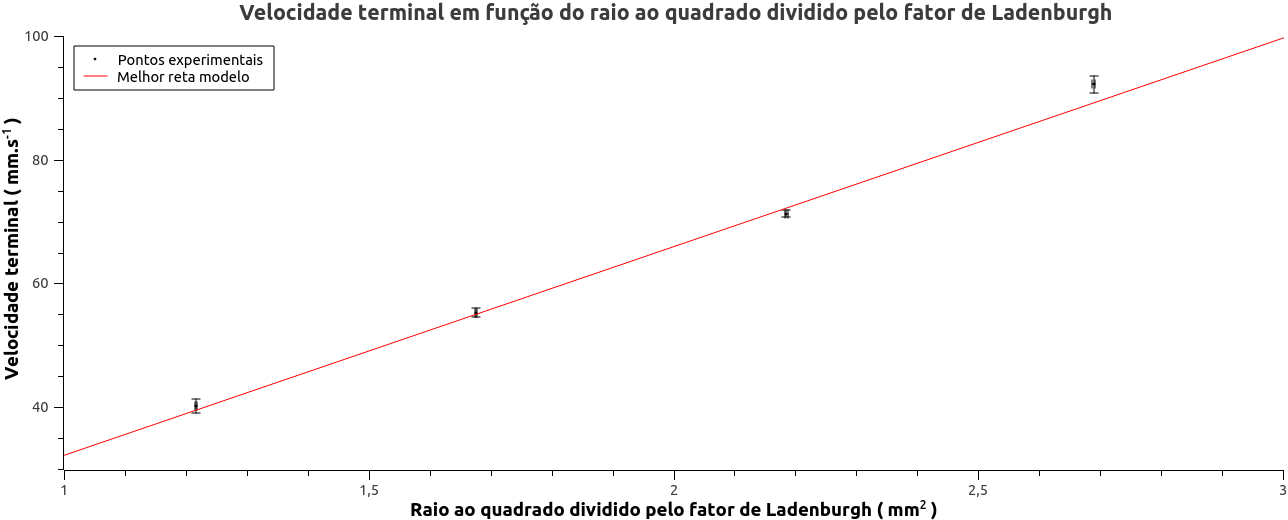
\includegraphics[scale = 0.30]{graph1.png}
		\caption{Gráfico com as incertezas.}
\end{figure}

%\begin{figure}[!h]
		%\centering
		%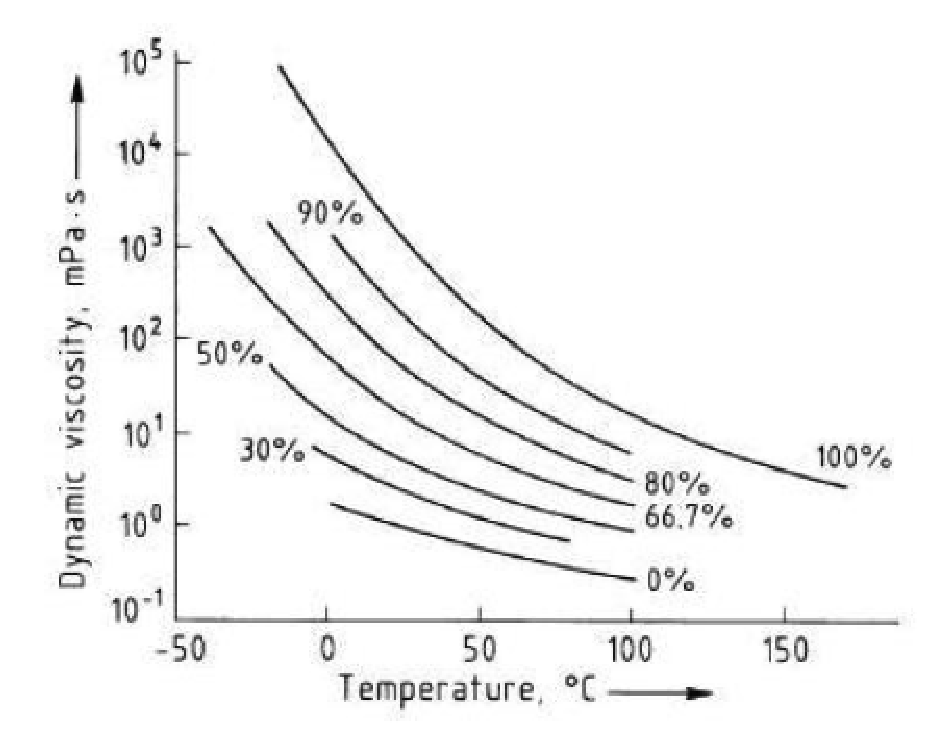
\includegraphics[scale = 0.4]{fig2.eps}
		%\caption{Viscosidade da mistura glicerina-água. As concentrações são dadas em percentual de massa de glicerina.}
		%\end{figure}

\paragraph{•}
Assim, achamos o coeficiente angular (a) sendo, $a = (34 +/- 1) mm^{-1} \cdot s^{-1}$. Logo obtemos o valor, $\eta = (428 +/- 13) mPa \cdot s$, para o coeficiente de viscosidade. 
Com o valor do coeficiente de viscosidade, com a temperatura do experimento $27 ºC$ e com auxílio da tabela dada pelo moodle, podemos descobrir o percentual de água na mistura. O valor obtido experimentalmente inclui um valor tabelado, $420 mPa\cdot s$, para a temperatura de 27,5 ºC. Logo podemos deduzir que o percentual de água como $3,11 \%$ e de glicerina, aproximadamente, $ 96,89\%$ - sem fazer a interpolação, visto que o valor encontrado reside nas imediações do tabelado. Se fizermos um gráfico sem barra de incerteza obteríamos um coeficiente angular muito semelhante.

\textbf{OBS}: Fizemos a análise da velocidade limite no Tracker. Os valores deram, estatisticamente, bem próximos dos medidos com cronômetro. Como exemplo, as velocidades de queda da esfera 2 deram, na média, $54 mm \cdot s^{-1}$.

	
		\end{enumerate}

	
\pagebreak

\textbf{Anexos}

\begin{figure}[!h]
		\centering
		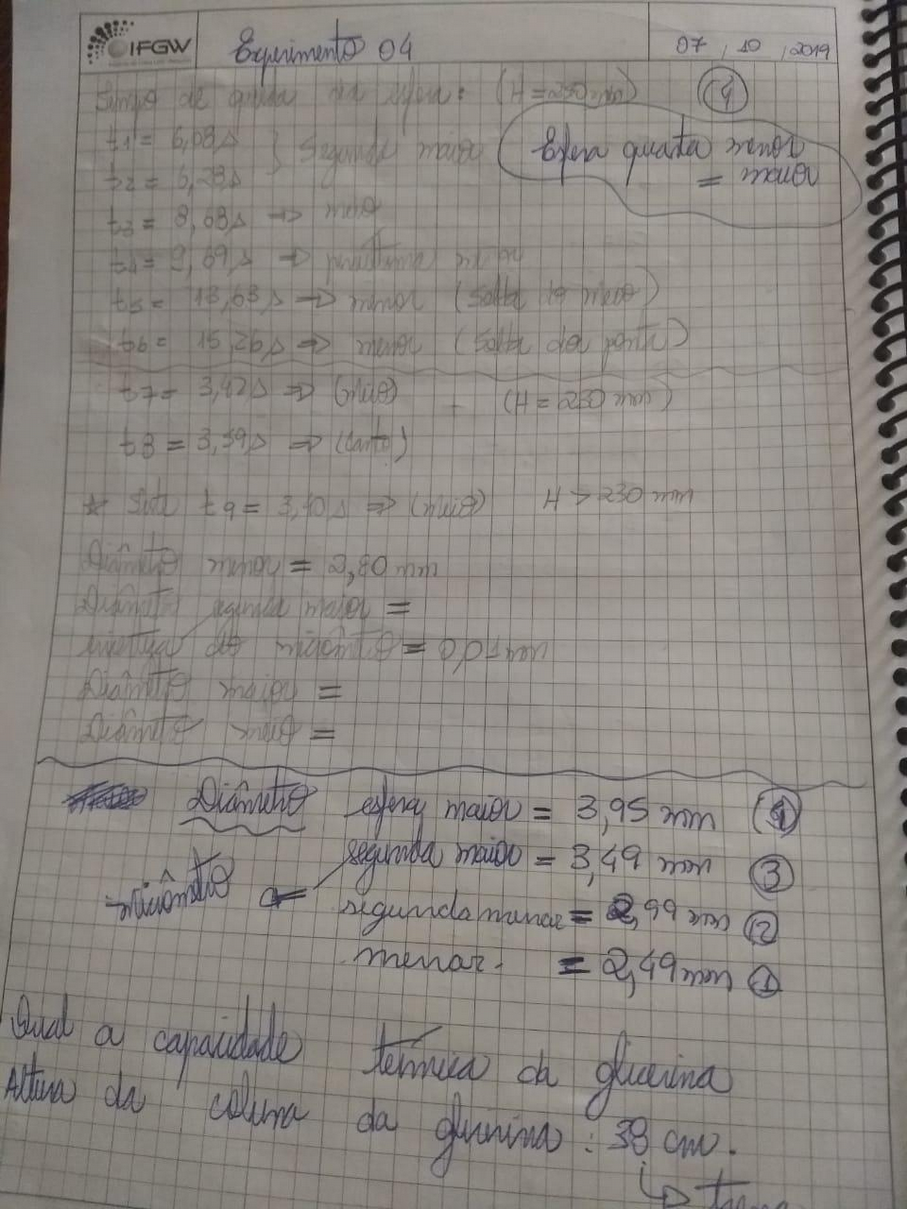
\includegraphics[scale = 0.50]{anexo1.png}
		%\caption{}
		\end{figure}

\begin{figure}[!h]
		\centering
		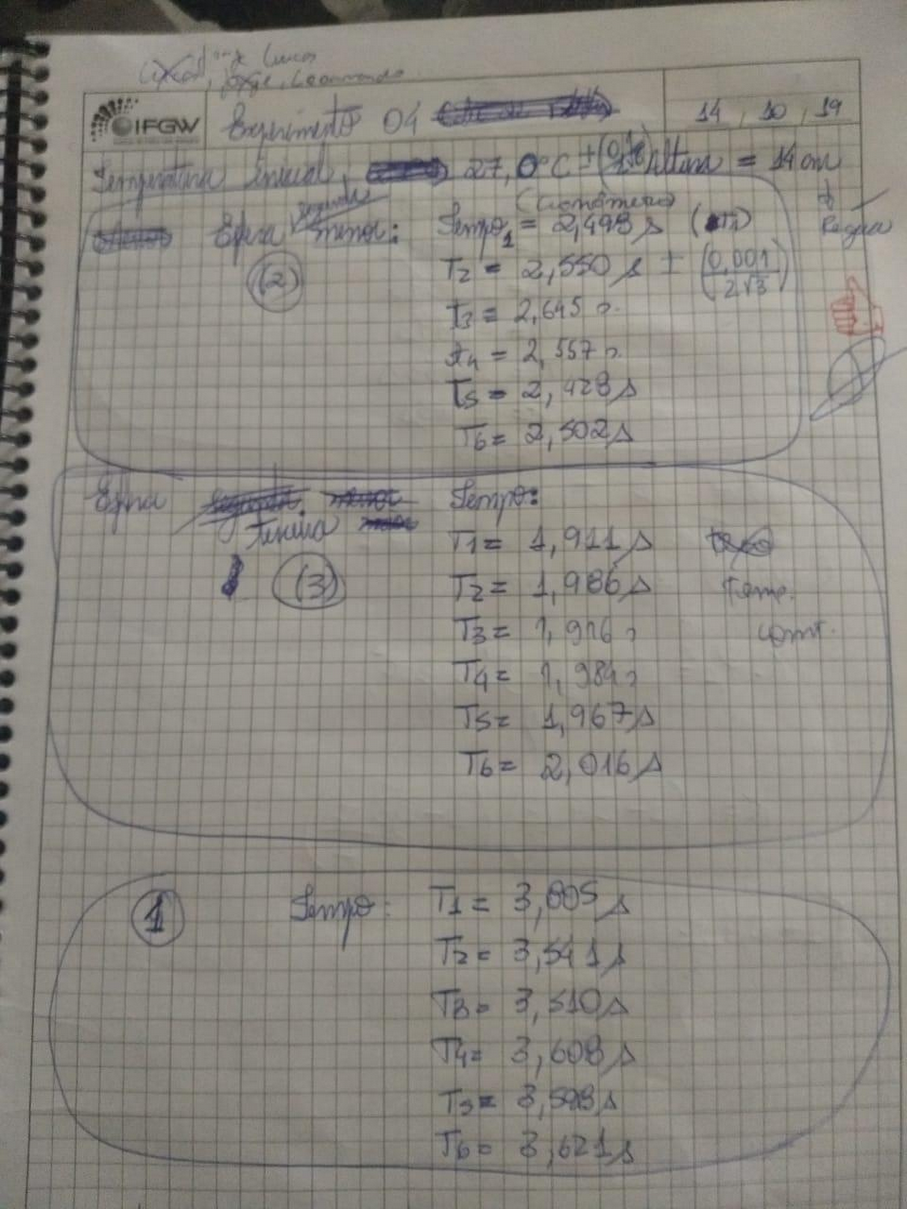
\includegraphics[scale = 0.50]{anexo2.png}
		%\caption{}
		\end{figure}

\begin{figure}[!h]
		\centering
		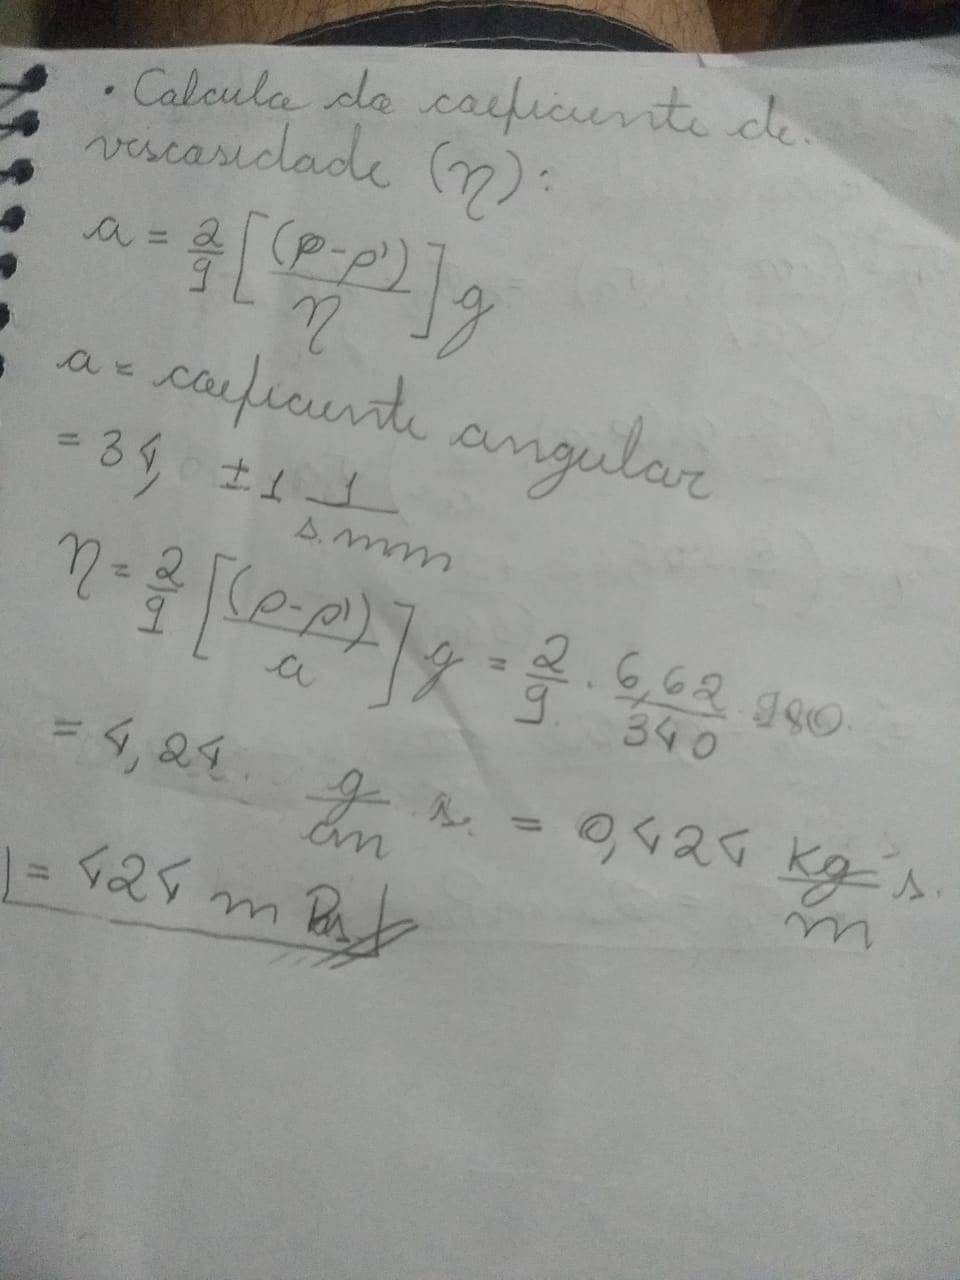
\includegraphics[scale = 0.50]{anexo3.png}
		%\caption{}
		\end{figure}


























%%%%%%%%%%%%%%%%%%%%%%%%%%%%%Fim do documento%%%%%%%%%%%%%%%%%%%%%%%%
\end{document}
